\section{Study setup}
\label{approach}
In this section, we present our case study setup. In particular, we present the datasets used in our case study and our experimental setup to collect ...

\subsection{Corpus construction}
AIDev dataset - LLM-based performance detection - 1,219 performance PRs across 447 repositories and five agents

The overview of datasets is shown in Table~\ref{dataset}.

\begin{table}
\centering
\caption{\shuang{Overview of datasets used in our study}}
\label{dataset}
\resizebox{0.9\columnwidth}{!}{  
\begin{tabular}{ccccc}
\toprule
Dataset   & Language & \#Instances & Year & Reference \\ \toprule
HumanEval & Python   & 164        & 2021 &      \cite{chen2021evaluating}    \\ 
AixBench  & Java     & 187        & 2022 &   \cite{hao2022aixbench}        \\ 
MBPP      & Python   & 974        & 2021  &   \cite{austin2021mbpp}       \\
EvalPerf  & Python   & 118        & 2024  &   \cite{DBLP:journals/corr/abs-2408-06450}       \\\bottomrule
\end{tabular}
}
\end{table}



\subsection{Experimental setup}
In this subsection, we describe the process of collecting the generated PRs and performance data for each question in our study datasets. Figure~\ref{overview} illustrates the overall process of our approach. We follow four steps to collect the needed data. In the first step, we .... 

\begin{figure*}[tbh]
\centerline{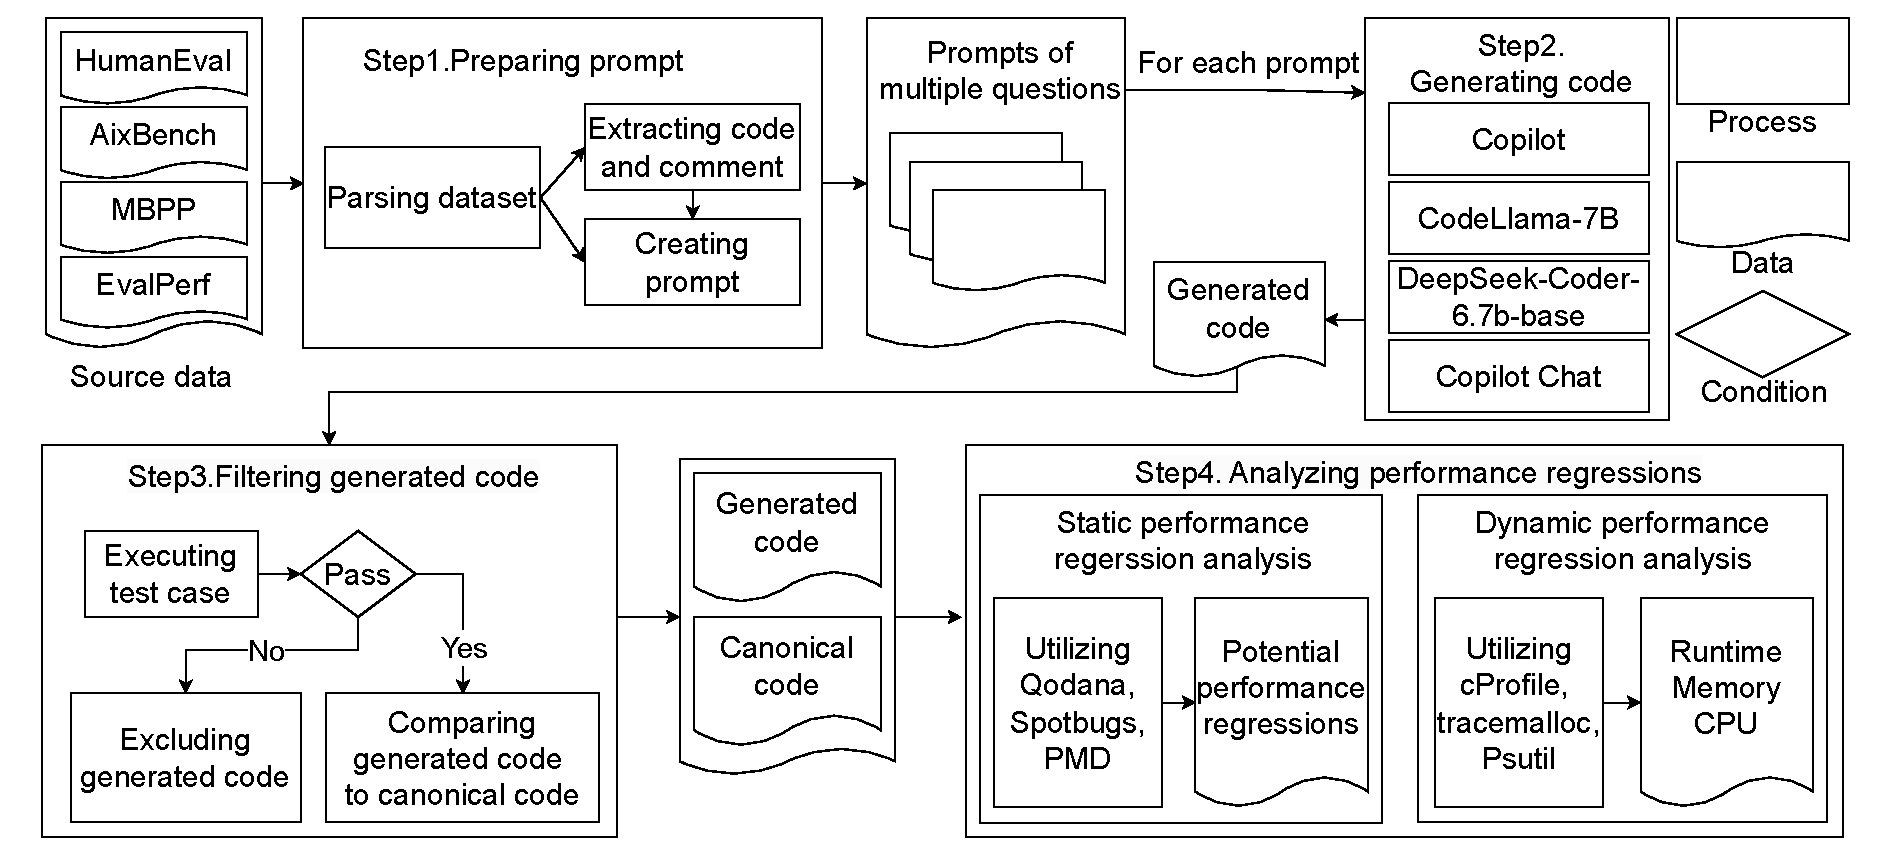
\includegraphics[width=1\textwidth]{./pics/approach/overview-new-new.drawio.pdf}}
\caption{\shuang{An overview of our approach to collecting data.}}
\label{overview}
\end{figure*}

{\textbf{Step 1: XXX.}} 


{\textbf{Step 2: Generating code.}}
In this step, we use

\textbf{Step 3. Filtering performance-related PRs.}
In this step, we filter 


\textbf{Step 4. Analyzing PR data.}
\label{analyze}

The hardware configuration for the experiment includes an Intel Core i9-13900K processor, 128 GB of RAM, 1 TB SSD for primary storage, and 8 TB HDD for secondary storage, and the system operates on Ubuntu 22.04.4 LTS. By following the experimental setup, we aim to achieve a thorough and systematic evaluation of the performance regressions of AI-generated code, considering both static and dynamic aspects, and providing actionable insights for code optimization and tool improvement.